\documentclass[10pt]{beamer}

\usetheme{metropolis}
\usepackage{appendixnumberbeamer}
\usepackage{caption}

\usepackage{booktabs}
\usepackage[scale=2]{ccicons}

\usepackage{pgfplots}
\usepgfplotslibrary{dateplot}

\usepackage{xspace}
\usepackage{chronology}
\usepackage{tabls}
\usepackage{tikz}
\usepackage{bchart}
\usepackage{appendixnumberbeamer}
\usepackage{outlines}

\newcommand{\themename}{\textbf{\textsc{metropolis}}\xspace}

\hypersetup{pdfpagemode=FullScreen}

\title{Linux}
\subtitle{Eine kurze Einführung}
\date{20. Mai 2019}
\author{Alex Neher}
\titlegraphic{\hfill
\includegraphics[height=1.5cm]{img/Tux.png}}

\begin{document}

\pagestyle{empty}
	
\begin{frame}

\end{frame}

\maketitle

\begin{frame}{Inhalt}
  \setbeamertemplate{section in toc}[sections numbered]
  \tableofcontents[hideallsubsections]
\end{frame}

\section{Was ist Linux?}

\begin{frame}{Was ist Linux?}
    \begin{itemize}[<+- | alert@+>]
        \item Betriebssystem/Kernel
        \item Meist verwendet für Server
        \item Android
    \end{itemize}

\end{frame}

\begin{frame}{Betriebssystem/Kernel}
    \centering
    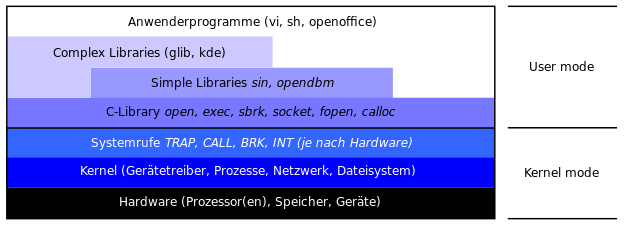
\includegraphics[keepaspectratio,width=0.9\textwidth]{img/kernel_schichten.png}
\end{frame}

\begin{frame}{GNU/Linux}
    \centering
    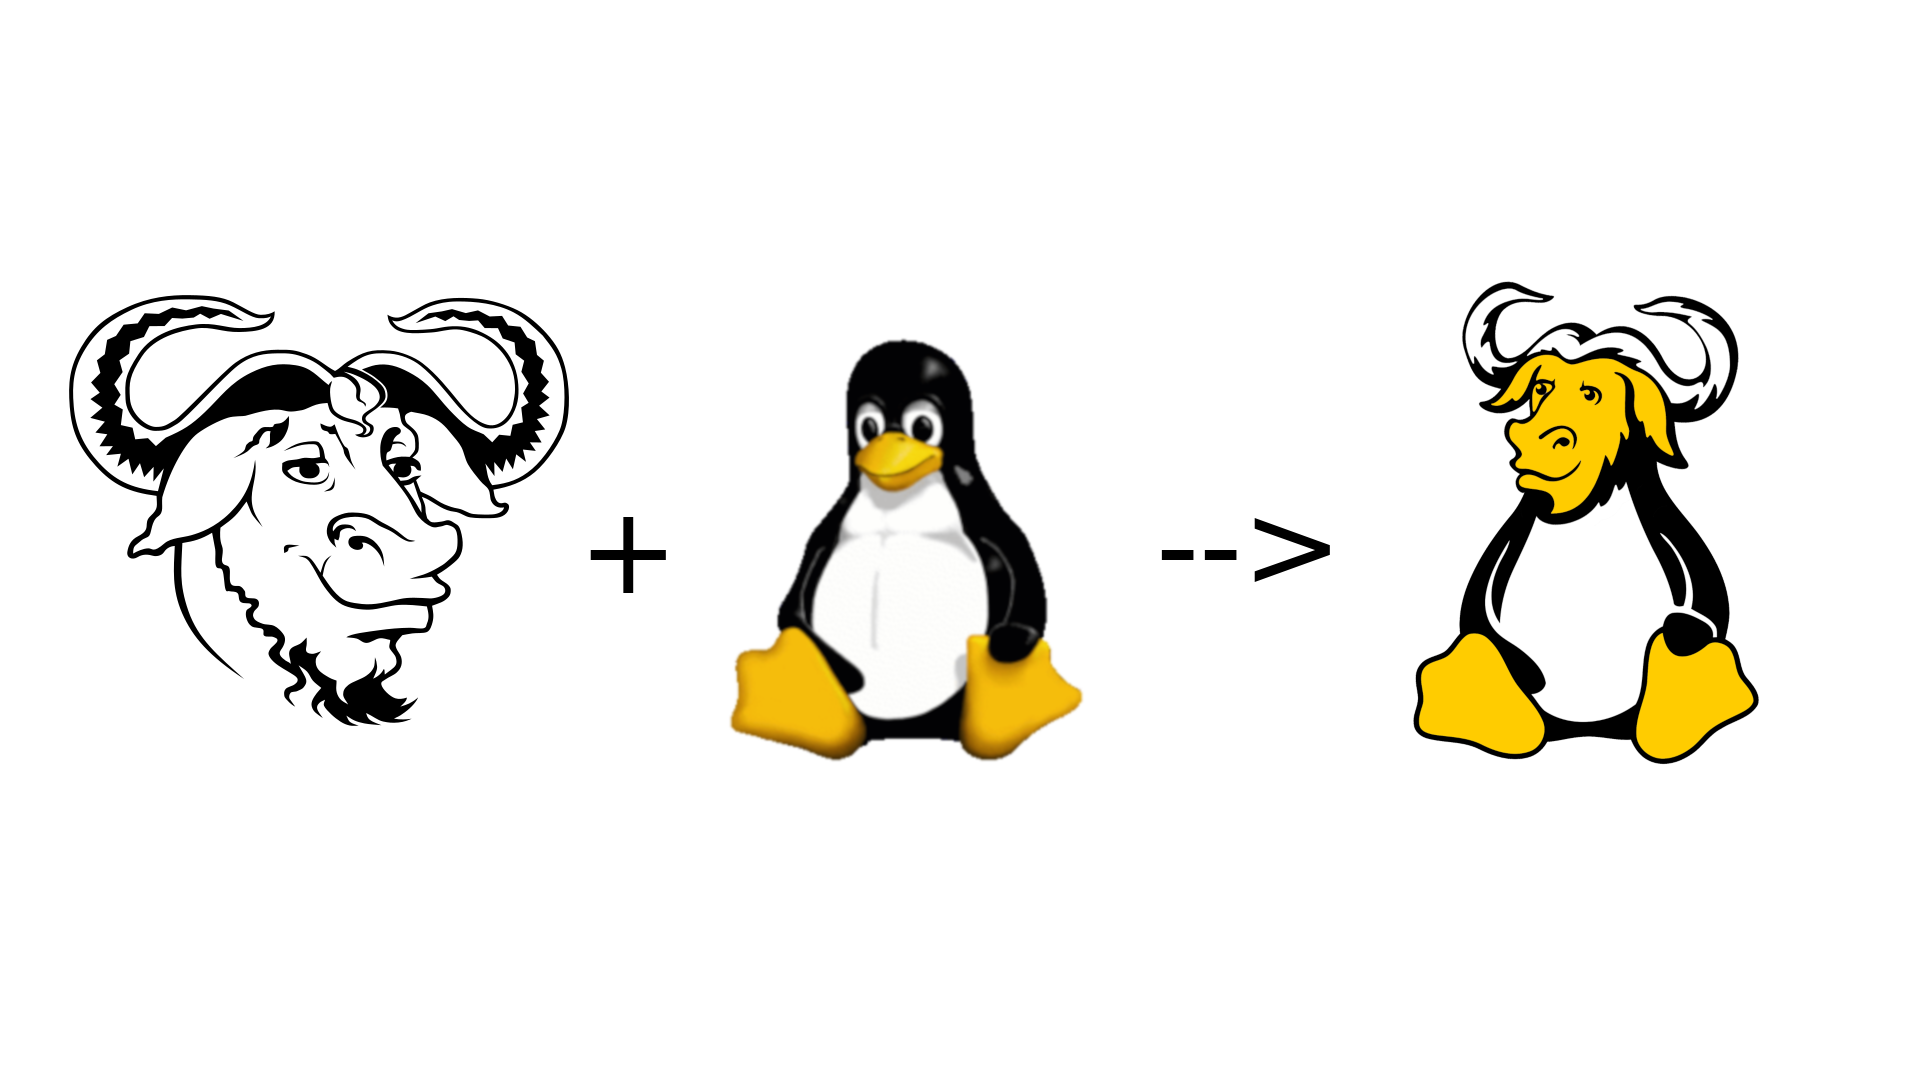
\includegraphics[keepaspectratio,width=0.9\textwidth]{img/gnupluslinux.png}
\end{frame}

\section{Freie Software}

\begin{frame}{Was ist "Free Software"?}
    \centering
    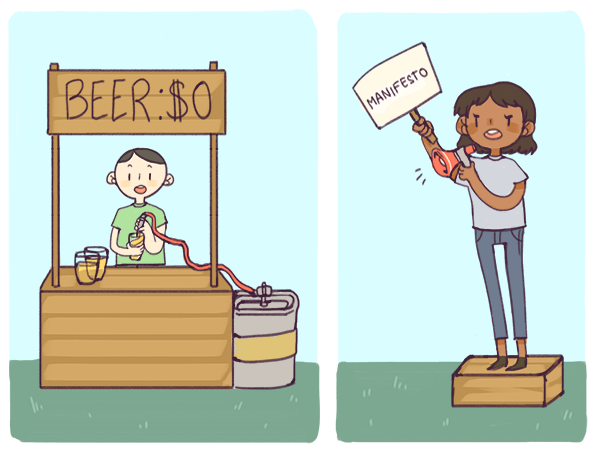
\includegraphics[keepaspectratio,width=0.9\textwidth]{img/freesoftware.png}
\end{frame}

\begin{frame}{Was ist "Free Software"?}
    \begin{columns}[T,onlytextwidth]
        \column{0.45\textwidth}
            \textbf{Free as in Beer}
            \begin{outline}
                \1 Gratis zum Herunterladen und Benutzen
                    \2 Adobe Flash Player
                    \2 Java
            \end{outline}
        \column{0.45\textwidth}
            \textbf{Free as in Speech}
            \begin{outline}
                \1 Respektiert die 'vier Freiheiten'
                    \2 GNU/Linux
                    \2 GIMP
            \end{outline}
    \end{columns}
\end{frame}

\begin{frame}{Die 'vier Freiheiten'}
    \begin{enumerate}
        \setcounter{enumi}{-1}
        \item Uneingeschränktes Verwenden zu jedem Zweck
        \item Das Recht, die Funktionsweise zu untersuchen und zu verstehen
        \item Das Recht, Kopien der Software zu verbreiten
        \item Das Recht, die Software zu verbessern und die Verbesserungen zu verbreiten
    \end{enumerate}
\end{frame}

\section{Linux im Alltag}

\begin{frame}{Software}
    \centering
    \includegraphics[keepaspectratio,width=\textwidth]{img/software.png}
\end{frame}

\begin{frame}{Distributionen}
    \centering
    
\includegraphics[keepaspectratio,width=0.9\textwidth]{img/logos_2.png}
\end{frame}

\begin{frame}{Desktopumgebungen}
\centering
\includegraphics[keepaspectratio,width=\textwidth]{img/desktops_2.png}
\end{frame}

\begin{frame}[standout]
Fragen?
\end{frame}

\end{document}
